% !TeX program = xelatex
\documentclass[a4paper,10pt]{article}

% ============================================================================
% កញ្ចប់សម្ភារៈសិក្សាបោះពុម្ព ស-ខ្មៅ (Printable Classroom Materials - Grade 8 RN1)
% ត្រូវគ្នា ១០០% នឹង LS_Plan_RN1.tex និង Teaching_Scenario_RN1.tex
% ហាមប្រើ \tiny, ហាមពណ៌ចម្រុះ, ខ្នាត 1:1 (x=1cm, y=1cm) ពិតប្រាកដលើទំព័រ ១
% ============================================================================
\usepackage[a4paper, left=1.0cm, right=1.0cm, top=0.75cm, bottom=1.05cm, footskip=0.55cm]{geometry}
\usepackage{amsmath, amssymb}
\usepackage{unicode-math}
\usepackage{fontspec}
\usepackage{array, colortbl}
\usepackage[table]{xcolor}
\usepackage{enumitem}
\usepackage{pifont}
\usepackage{fancyhdr}
\usepackage{lastpage}
\usepackage{tikz}
\usepackage[most]{tcolorbox}
\usetikzlibrary{calc, arrows.meta, positioning, babel}

% LaTeX 2025 compatibility guard
\makeatletter
\let\@expl@@@mark@update@singlecol@structures@@\relax
\makeatother

% ============================================================================
% ការកំណត់ពុម្ពអក្សរផ្លូវការ (Cross-Platform Windows + Cloud fonts/)
% ============================================================================
\providecommand{\NGSFindFonts}{%
  \IfFileExists{C:/Windows/Fonts/cambria.ttc}{%
    \def\NGSSysPath{C:/Windows/Fonts/}%
    \def\NGSUserPath{C:/Users/KIT/AppData/Local/Microsoft/Windows/Fonts/}%
  }{%
    \IfFileExists{./fonts/KhmerOSsiemreap.ttf}{\def\NGSSysPath{./fonts/}\def\NGSUserPath{./fonts/}}{%
    \IfFileExists{../fonts/KhmerOSsiemreap.ttf}{\def\NGSSysPath{../fonts/}\def\NGSUserPath{../fonts/}}{%
    \IfFileExists{../../fonts/KhmerOSsiemreap.ttf}{\def\NGSSysPath{../../fonts/}\def\NGSUserPath{../../fonts/}}{%
    \IfFileExists{../../../fonts/KhmerOSsiemreap.ttf}{\def\NGSSysPath{../../../fonts/}\def\NGSUserPath{../../../fonts/}}{%
    \IfFileExists{../../../../fonts/KhmerOSsiemreap.ttf}{\def\NGSSysPath{../../../../fonts/}\def\NGSUserPath{../../../../fonts/}}{%
    \IfFileExists{../../../../../fonts/KhmerOSsiemreap.ttf}{\def\NGSSysPath{../../../../../fonts/}\def\NGSUserPath{../../../../../fonts/}}{%
    \IfFileExists{../../../../../../fonts/KhmerOSsiemreap.ttf}{\def\NGSSysPath{../../../../../../fonts/}\def\NGSUserPath{../../../../../../fonts/}}{%
      \def\NGSSysPath{../../../../../../../fonts/}\def\NGSUserPath{../../../../../../../fonts/}%
    }}}}}}}%
  }%
}
\NGSFindFonts

\setmathfont[
  Path={\NGSSysPath},
  FontIndex=1,
  Scale=1.02
]{cambria.ttc}

\defaultfontfeatures{Ligatures=TeX}

\setmainfont[
  Path={\NGSUserPath},
  Extension=.ttf,
  Script=Khmer,
  BoldFont={KhmerOSsiemreap},
  BoldFeatures={FakeBold=1.8},
  ItalicFont={KhmerOSsiemreap},
  ItalicFeatures={FakeSlant=0.25},
  BoldItalicFont={KhmerOSsiemreap},
  BoldItalicFeatures={FakeBold=1.8, FakeSlant=0.25}
]{KhmerOSsiemreap}

\newfontfamily\muol[
  Path={\NGSUserPath},
  Extension=.ttf,
  Script=Khmer
]{KhmerOSmuollight}

\newfontfamily\TimesEn[
  Path={\NGSSysPath},
  Extension=.ttf,
  BoldFont={timesbd},
  ItalicFont={timesi},
  BoldItalicFont={timesbi}
]{times}

\newfontfamily\CalibriFont[
  Path={\NGSSysPath},
  Extension=.ttf
]{calibri}

\newfontfamily\Tacteing[
  Path={\NGSUserPath}
]{TACTENG.TTF}

\XeTeXlinebreaklocale "km"
\XeTeXlinebreakskip = 0pt plus 1pt minus 0.1pt

% ============================================================================
% ក្ដារពណ៌ ស-ខ្មៅ សុទ្ធសម្រាប់ការបោះពុម្ព (Strict Monochrome Print Palette)
% ============================================================================
\definecolor{panelgray}{gray}{0.92} % gray!8
\definecolor{headgray}{gray}{0.85}  % gray!15
\definecolor{midgray}{gray}{0.75}   % gray!25
\definecolor{darkline}{gray}{0.35}  % gray!65

\pagestyle{fancy}
\fancyhf{}
\renewcommand{\headrulewidth}{0pt}
\fancyfoot[L]{\fontsize{8.0pt}{10.5pt}\selectfont អនុវិទ្យាល័យព្រះក្រសាំង \en{—} គណិតវិទ្យា ថ្នាក់ទី៨ \en{|} មេរៀនទី១ (១. សញ្ញាណចំនួនសនិទាន) ស-ខ្មៅ \en{|} ថ្ងៃចន្ទ ៨រោច អស្សុជ ២៥៧០ \en{|} ថ្ងៃទី២ ខែវិច្ឆិកា ឆ្នាំ២០២៦}
\fancyfoot[R]{\fontsize{8.3pt}{10.5pt}\selectfont ទំព័រ \en{\thepage\ / \pageref{LastPage}}}

\setlength{\parindent}{0pt}
\setlength{\parskip}{0pt}
\setlength{\tabcolsep}{4pt}

% ============================================================================
% ម៉ាក្រូជំនួយ (Helper Macros)
% ============================================================================
\newcommand{\en}[1]{{\TimesEn #1}}
\newcommand{\enbf}[1]{{\TimesEn\textbf{#1}}}
\newcommand{\unit}[1]{\,\text{\en{#1}}}
\newcommand{\cnum}[1]{\mbox{\fontsize{10pt}{12pt}\selectfont\ding{\numexpr181+#1\relax}}}
\newcommand{\scissors}{\ding{34}}
\newcommand{\chkbox}{\tikz[baseline=-0.15ex]\draw[black, line width=0.9pt] (0,0) rectangle (0.24cm,0.24cm);}
\newcommand{\khmflourish}{{\Tacteing\fontsize{32pt}{13pt}\selectfont\raisebox{-4pt}{3}}}
\newcommand{\fnum}[1]{\text{\raisebox{1.5pt}{\makebox[#1]{\dotfill}}}}
\newcommand{\fden}[1]{\text{\makebox[#1]{\dotfill}}}

\newcommand{\pagebanner}[2]{%
  \begin{tcolorbox}[
    enhanced, sharp corners, colback=headgray, colframe=black,
    boxrule=1.1pt, boxsep=1pt, top=3pt, bottom=3pt, left=6pt, right=6pt,
    after skip=4pt
  ]
    {\muol\fontsize{9.2pt}{13.5pt}\selectfont #1}\hfill{\fontsize{8.2pt}{11.5pt}\selectfont\textbf{#2}}
  \end{tcolorbox}%
}

\newcolumntype{L}[1]{>{\raggedright\arraybackslash}p{#1}}
\newcolumntype{C}[1]{>{\centering\arraybackslash}p{#1}}

\begin{document}
\fontsize{9.0pt}{13.2pt}\selectfont

% ============================================================================
% ទំព័រទី ១៖ សម្ភារៈ E2 ខ្នាតពិត 1:1 (បន្ទះកាត់ 6.00 cm = 1 unit, បន្ទាត់ភ្លោះ, POE 2A-2B)
% ============================================================================
\pagebanner{សម្ភារៈទី ១៖ បន្ទះបត់ \enbf{E2} ខ្នាតពិត \enbf{1:1} \enbf{(1} ឯកតា \enbf{= 6.00 cm)} \enbf{\&} ពិសោធន៍ \enbf{POE 2A–2B}}{ទំព័រ ១/៦ \en{– E2 Explore}}

% --- ប្រអប់ព្រមាន Actual Size 100% + បន្ទះផ្ទៀង 5.00 cm (x=1cm, y=1cm) ---
\noindent
\begin{minipage}[c]{11.8cm}
  \begin{tcolorbox}[
    enhanced, sharp corners, colback=panelgray, colframe=black,
    boxrule=1.0pt, boxsep=1pt, top=3pt, bottom=3pt, left=6pt, right=6pt
  ]
    \fontsize{8.2pt}{11.5pt}\selectfont
    \textbf{ការណែនាំមុនបោះពុម្ព (\en{Print at 100\% / Actual Size})៖} ត្រូវជ្រើស \textbf{\en{Scale: Actual Size 100\%}} \en{–} \textbf{ហាម \en{Fit to Page}} ដើម្បីឱ្យបន្ទះបត់ទាំង ៤ ($1\text{ ឯកតា} = 6.00\unit{cm}$) និងបន្ទាត់ភ្លោះ $[-1.5, +1.5]$ ($18.00\unit{cm}$) មានខ្នាតពិត \en{1:1}។\\[2pt]
    \textbf{«ក្រុមវិស្វករសហគមន៍»៖} កាត់ \scissors{} បន្ទះ ៤ ខាងក្រោម បត់ជា $2$, $3$, $4$ ផ្នែកស្មើ រួចផ្ទៀងលើបន្ទាត់ភ្លោះ!
  \end{tcolorbox}
\end{minipage}%
\hfill
\begin{minipage}[c]{6.9cm}
  \begin{tcolorbox}[
    enhanced, sharp corners, colback=white, colframe=black,
    boxrule=1.0pt, boxsep=1pt, top=2.5pt, bottom=2.5pt, left=4pt, right=4pt
  ]
    \centering
    {\fontsize{8.0pt}{10.5pt}\selectfont\textbf{បន្ទះផ្ទៀងខ្នាតពិត \en{5.00 cm} (\en{Actual Size 100\%})}}\\[2pt]
    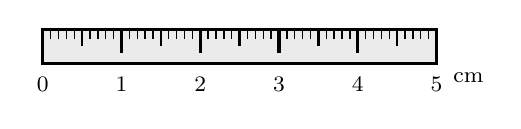
\begin{tikzpicture}[x=1cm, y=1cm, every node/.style={font=\footnotesize, text=black}]
      \draw[black, line width=1.1pt, fill=panelgray] (0,0) rectangle (5.0, 0.44);
      \foreach \m in {0,...,50}{
        \pgfmathsetmacro{\xval}{\m*0.1}
        \draw[black, line width=0.5pt] (\xval, 0.44) -- (\xval, 0.32);
      }
      \foreach \h in {0,0.5,...,5.0}{
        \draw[black, line width=0.85pt] (\h, 0.44) -- (\h, 0.23);
      }
      \foreach \c in {0,1,2,3,4,5}{
        \draw[black, line width=1.15pt] (\c, 0.44) -- (\c, 0.14);
        \node[below=1pt] at (\c, 0.0) {\en{\c}};
      }
      \node[right=2pt] at (5.02, -0.18) {\en{cm}};
    \end{tikzpicture}
  \end{tcolorbox}
\end{minipage}

\vspace{4pt}

% --- ផ្នែកទី ១៖ បន្ទះបត់ 1:1 (៤ បន្ទះ × 6.00 cm) + បន្ទាត់ភ្លោះ [-1.5, +1.5] ---
\textbf{១. សកម្មភាព \en{1} ៖ កាត់បន្ទះបត់ខ្នាត \en{1:1} ($1\text{ ឯកតា} = 6.00\unit{cm}$ ពិត) ដាក់ផ្ទៀងលើបន្ទាត់ភ្លោះ $[-1.5, +1.5]$ (\en{x=1cm, y=1cm})}

\vspace{2pt}
\noindent
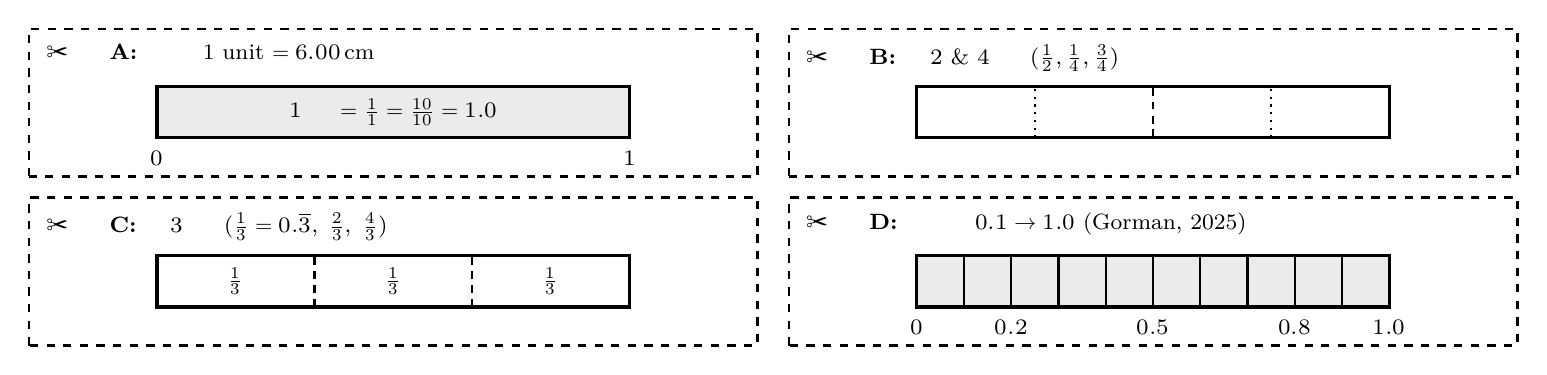
\begin{tikzpicture}[x=1cm, y=1cm, every node/.style={font=\footnotesize, text=black}]
  % === ROW 1: Strip A (Whole 6.00cm) & Strip B (Fold 2 & 4, 6.00cm) ===
  % Cut box A (0..9.25, 2.35..4.22)
  \draw[black, dashed, line width=0.95pt] (0, 2.35) rectangle (9.25, 4.22);
  \node[anchor=north west] at (0.10, 4.15) {\scissors\ \textbf{កាត់ \en{A}:} បន្ទះពេញ \en{1 unit} $= 6.00\unit{cm}$};
  \draw[black, line width=1.2pt, fill=panelgray] (1.625, 2.84) rectangle (7.625, 3.49);
  \node at (4.625, 3.165) {$1\text{ ឯកតា} = \frac{1}{1} = \frac{10}{10} = 1.0$};
  \node[anchor=north] at (1.625, 2.80) {$0$};
  \node[anchor=north] at (7.625, 2.80) {$1$};

  % Cut box B (9.65..18.90, 2.35..4.22)
  \draw[black, dashed, line width=0.95pt] (9.65, 2.35) rectangle (18.90, 4.22);
  \node[anchor=north west] at (9.75, 4.15) {\scissors\ \textbf{កាត់ \en{B}:} បត់ $2$ \& $4$ ស្មើ ($\frac{1}{2}, \frac{1}{4}, \frac{3}{4}$)};
  \draw[black, line width=1.2pt, fill=white] (11.275, 2.84) rectangle (17.275, 3.49);
  \draw[black, densely dashed, line width=0.9pt] (14.275, 2.84) -- (14.275, 3.49);
  \draw[black, dotted, line width=0.8pt] (12.775, 2.84) -- (12.775, 3.49);
  \draw[black, dotted, line width=0.8pt] (15.775, 2.84) -- (15.775, 3.49);
  \node[fill=white, inner sep=1pt] at (14.275, 3.165) {បត់តាមស្នាមចុច};

  % === ROW 2: Strip C (Fold 3, 6.00cm) & Strip D (Decimal 10ths, 6.00cm) ===
  % Cut box C (0..9.25, 0.20..2.08)
  \draw[black, dashed, line width=0.95pt] (0, 0.20) rectangle (9.25, 2.08);
  \node[anchor=north west] at (0.10, 2.01) {\scissors\ \textbf{កាត់ \en{C}:} បត់ $3$ ស្មើ ($\frac{1}{3}=0.\overline{3},\; \frac{2}{3},\; \frac{4}{3}$)};
  \draw[black, line width=1.2pt, fill=white] (1.625, 0.69) rectangle (7.625, 1.34);
  \draw[black, densely dashed, line width=0.9pt] (3.625, 0.69) -- (3.625, 1.34);
  \draw[black, densely dashed, line width=0.9pt] (5.625, 0.69) -- (5.625, 1.34);
  \node at (2.625, 1.015) {$\frac{1}{3}$};
  \node at (4.625, 1.015) {$\frac{1}{3}$};
  \node at (6.625, 1.015) {$\frac{1}{3}$};

  % Cut box D (9.65..18.90, 0.20..2.08)
  \draw[black, dashed, line width=0.95pt] (9.65, 0.20) rectangle (18.90, 2.08);
  \node[anchor=north west] at (9.75, 2.01) {\scissors\ \textbf{កាត់ \en{D}:} បន្ទះទសភាគ $0.1 \to 1.0$ (\en{Gorman, 2025})};
  \draw[black, line width=1.2pt, fill=panelgray] (11.275, 0.69) rectangle (17.275, 1.34);
  \foreach \k in {1,...,9}{
    \pgfmathsetmacro{\tx}{11.275 + 0.6*\k}
    \draw[black, line width=0.75pt] (\tx, 0.69) -- (\tx, 1.34);
  }
  \node[anchor=north] at (11.275, 0.65) {$0$};
  \node[anchor=north] at (12.475, 0.65) {$0.2$};
  \node[anchor=north] at (14.275, 0.65) {$0.5$};
  \node[anchor=north] at (16.075, 0.65) {$0.8$};
  \node[anchor=north] at (17.275, 0.65) {$1.0$};
\end{tikzpicture}

\vspace{3pt}
\noindent
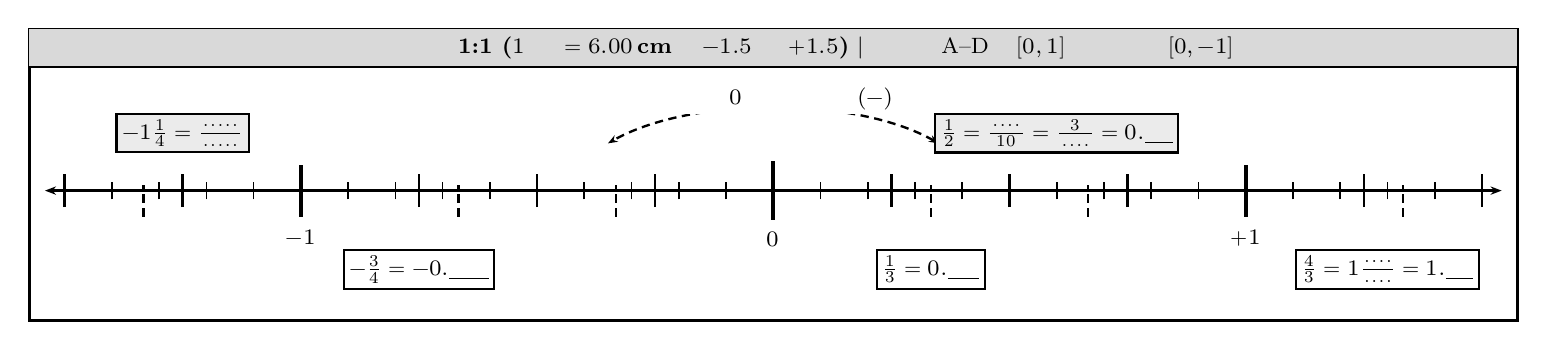
\begin{tikzpicture}[x=1cm, y=1cm, every node/.style={font=\footnotesize, text=black}]
  % === Unified 1:1 Twin Number Line Mat [-1.5, +1.5], 1 unit = 6.00 cm ===
  % Frame: 18.90 cm wide, center 0 at x = 9.45 -> -1.5 at 0.45, -1 at 3.45, +1 at 15.45, +1.5 at 18.45
  \draw[black, line width=1.1pt] (0, 0) rectangle (18.90, 3.70);
  \fill[headgray] (0, 3.22) rectangle (18.90, 3.70);
  \draw[black, line width=0.85pt] (0, 3.22) -- (18.90, 3.22);
  \node at (9.45, 3.46) {\textbf{បន្ទាត់ចំនួនភ្លោះខ្នាត \en{1:1} ($1\text{ ឯកតា} = 6.00\unit{cm}$ ពី $-1.5$ ដល់ $+1.5$)} \textbar\ ផ្ទៀងបន្ទះ \en{A–D} លើ $[0,1]$ រួចត្រឡប់ឆ្វេង $[0,-1]$};

  % Number line axis at y = 1.65
  \draw[{Stealth[length=4pt]}-{Stealth[length=4pt]}, black, line width=1.2pt] (0.20, 1.65) -- (18.70, 1.65);

  % Tenth ticks (0.60 cm)
  \foreach \i in {-14,...,14}{
    \pgfmathsetmacro{\xp}{9.45 + 0.6*\i}
    \draw[black, line width=0.6pt] (\xp, 1.54) -- (\xp, 1.76);
  }
  % Quarter ticks (1.50 cm)
  \foreach \q in {-6,-5,-3,-2,-1,1,2,3,5,6}{
    \pgfmathsetmacro{\xq}{9.45 + 1.5*\q}
    \draw[black, line width=0.9pt] (\xq, 1.44) -- (\xq, 1.86);
  }
  % Third ticks (2.00 cm) downwards highlight
  \foreach \t in {-4,-2,-1,1,2,4}{
    \pgfmathsetmacro{\xt}{9.45 + 2.0*\t}
    \draw[black, densely dashed, line width=0.85pt] (\xt, 1.32) -- (\xt, 1.72);
  }
  % Major integer ticks: -1 (3.45), 0 (9.45), +1 (15.45)
  \draw[black, line width=1.35pt] (3.45, 1.32) -- (3.45, 1.98);
  \node[below=3pt, fill=white, inner sep=1pt] at (3.45, 1.30) {\textbf{$-1$}};
  \draw[black, line width=1.45pt] (9.45, 1.28) -- (9.45, 2.02);
  \node[below=3pt, fill=white, inner sep=1pt] at (9.45, 1.28) {\textbf{$0$}};
  \draw[black, line width=1.35pt] (15.45, 1.32) -- (15.45, 1.98);
  \node[below=3pt, fill=white, inner sep=1pt] at (15.45, 1.30) {\textbf{$+1$}};

  % Negative mirror curved arrow from [0,1] to [0,-1]
  \draw[black, densely dashed, line width=0.85pt, {Stealth[length=3.5pt]}-{Stealth[length=3.5pt]}] (11.55, 2.25) .. controls (10.50, 2.85) and (8.40, 2.85) .. (7.35, 2.25);
  \node[fill=white, inner sep=1.5pt] at (9.45, 2.82) {ត្រឡប់ឆ្វេង $0$ ជាចំនួនអវិជ្ជមាន ($-$)};

  % Target student callout blanks clearly positioned without touching
  \node[draw=black, line width=0.75pt, fill=panelgray, inner sep=2pt] at (1.95, 2.38) {$-1\frac{1}{4} = \frac{\fnum{0.50cm}}{\fden{0.50cm}}$};
  \node[draw=black, line width=0.75pt, fill=white, inner sep=2pt] at (4.95, 0.65) {$-\frac{3}{4} = -0.\underline{\hspace{0.5cm}}$};
  \node[draw=black, line width=0.75pt, fill=white, inner sep=2pt] at (11.45, 0.65) {$\frac{1}{3} = 0.\underline{\hspace{0.4cm}}$};
  \node[draw=black, line width=0.75pt, fill=panelgray, inner sep=2pt] at (13.05, 2.38) {$\frac{1}{2} = \frac{\fnum{0.42cm}}{10} = \frac{3}{\fden{0.42cm}} = 0.\underline{\hspace{0.35cm}}$};
  \node[draw=black, line width=0.75pt, fill=white, inner sep=2pt] at (17.25, 0.65) {$\frac{4}{3} = 1\frac{\fnum{0.38cm}}{\fden{0.38cm}} = 1.\underline{\hspace{0.35cm}}$};
\end{tikzpicture}

\vspace{4pt}

% --- ផ្នែកទី ២៖ Dual POE 2A & 2B Recording Sheet ---
\textbf{២. សកម្មភាព \en{2} (\en{POE 2A \& 2B}) ៖ អន្ទាក់លេខ ០, បឋមនឹងគ្នា vs កត្តា $\{2,5\}$, និងចំរុះដក ($-3\frac{1}{4}$)}

\vspace{2pt}
\begin{tcolorbox}[
  enhanced, sharp corners, colback=white, colframe=black,
  boxrule=1.05pt, boxsep=1pt, top=5pt, bottom=5pt, left=6pt, right=6pt
]
  \raggedright\fontsize{8.2pt}{11.8pt}\selectfont
  \textbf{\en{P} – ទស្សន៍ទាយមុនដោះស្រាយ (\en{Predict})៖}\\[2.5pt]
  \textbf{១) (\en{POE 2A})} តើ $\frac{0}{4}$, $\frac{4}{0}$ និង $\frac{0}{0}$ មួយណាស្មើ $0$? មួយណាគ្មានន័យ? \quad \chkbox~$\frac{0}{4}=0$ \quad \chkbox~$\frac{4}{0}=0$ \quad \chkbox~$\frac{4}{0}$ គ្មានន័យ\\[2.5pt]
  \textbf{២) (\en{POE 2B})} សៀវភៅទំ.១ ថាបឋមនឹងគ្នា $\to$ ខួប។ តើ $\frac{1}{2}$ បឋមនឹងគ្នាខួបឬដាច់? ចុះ $-3\frac{1}{4}$ ស្មើ $\frac{-13}{4}$ ឬ $\frac{-11}{4}$?\\[4pt]

  \textbf{\en{O} – តារាងសង្កេត និងផ្ទៀងផ្ទាត់ (\en{Observe})៖}\\[3pt]
  \renewcommand{\arraystretch}{1.24}
  \begin{tabular}{|L{3.90cm}|L{9.40cm}|L{4.05cm}|}
    \hline
    \cellcolor{headgray}\textbf{ពិសោធន៍ \en{POE}} & \cellcolor{headgray}\textbf{ការផ្ទៀងផ្ទាត់តាមច្រាសផលគុណ និងកត្តាបឋម} & \cellcolor{headgray}\textbf{សន្និដ្ឋាន (\en{Explain})} \\ \hline
    \textbf{\en{POE 2A}}៖ អន្ទាក់សូន្យ\par (\en{Karakuş \& Aydın, 2019}) &
    $\bullet\ \dfrac{0}{4}=k \iff k\times 4=0 \Rightarrow k = \underline{\hspace{0.55cm}}$ (\chkbox~មាន $1$ តម្លៃ)\par
    $\bullet\ \dfrac{4}{0}=k \iff k\times 0=4$ (\chkbox~គ្មាន $k$ ណាគុណ $0$ បាន $4$!) \;\textbar{}\; $\dfrac{0}{0}$: $k$ រាប់មិនអស់ &
    ហាម $b=0$ ដាច់ខាត៖\par
    \textbf{លក្ខខណ្ឌ $\underline{\hspace{1.4cm}}$ (\cnum{1})} \\ \hline
    \textbf{\en{POE 2B}}៖ ខួប vs $\{2,5\}$\par និងសញ្ញា $-3\frac{1}{4}$ &
    $\bullet\ \dfrac{1}{2} = \underline{\hspace{0.6cm}}$ (បឋមនឹងគ្នា តែដាច់!) \;\textbar{}\; $\dfrac{1}{3} = 0.\overline{3}$ (កត្តា $3 \notin \{2,5\}$)\par
    $\bullet\ -3\dfrac{1}{4} = -\!\left(3 + \dfrac{1}{4}\right) = \dfrac{\fnum{0.70cm}}{4}$ \;\textbar{}\; ហាម $\dfrac{-3\times 4+1}{4}=\dfrac{-11}{4}$ (\ding{55}) &
    ដាច់ $\iff$ កត្តា $\{2,5\}$;\par
    $-3\frac{1}{4} = \underline{\hspace{0.85cm}}$ (\cnum{3}) \\ \hline
  \end{tabular}\\[4pt]

  \textbf{\en{E} – សង្ខេបក្រុម (\en{Explain})៖} ចំនួនសនិទានមានទម្រង់ $\dfrac{a}{b}$ ដែល $a,b \in \mathbb{Z}$ និង $\underline{\hspace{1.2cm}}$ ហើយ $\dfrac{a}{b}=\dfrac{c}{d} \iff \underline{\hspace{1.8cm}}\;(b,d\neq 0)$~។
\end{tcolorbox}

\clearpage

% ============================================================================
% ទំព័រទី ២៖ E4 Elaborate — ២ ប័ណ្ណ «៣ ជំហានស៊ើបអង្កេត & [tracing]» (2-up)
% ============================================================================
\pagebanner{សម្ភារៈទី ២៖ កាត \enbf{E4} «៣ ជំហានស៊ើបអង្កេត \enbf{\& [tracing]}» \enbf{(}ទំ\enbf{.}២\enbf{)}}{ទំព័រ ២/៦ \en{– E4} (\scissors\ ២ ប័ណ្ណ)}

\newcommand{\eFourCardRN}[1]{%
\begin{tcolorbox}[
  enhanced, sharp corners, colback=white, colframe=white,
  borderline={1.0pt}{0pt}{black, dashed},
  boxsep=1pt, top=6.5pt, bottom=6.5pt, left=5pt, right=5pt
]
  \begin{tcolorbox}[
    enhanced, sharp corners, colback=headgray, colframe=black,
    boxrule=0.8pt, boxsep=1pt, top=3.5pt, bottom=3.5pt, left=5pt, right=5pt, after skip=6pt
  ]
    \fontsize{8.5pt}{11.6pt}\selectfont
    \textbf{\scissors\ កាត \en{E4} (#1) \en{–} លំហាត់គំរូទី \en{1} \& ទី \en{2} (ទំ.២ កែបំពេញ)} \hfill ក្រុម៖ $\underline{\hspace{2.8cm}}$
  \end{tcolorbox}

  \noindent
  \begin{minipage}[t]{7.50cm}
    \vspace{0pt}
    \fontsize{8.1pt}{11.6pt}\selectfont
    \textbf{គំរូទី ១ (ទំ.២)៖} ផ្គុំចំនួនស្មើគ្នាក្នុងបញ្ជី៖\\[3pt]
    \centerline{$-3\frac{1}{2},\quad 3.5,\quad \frac{-7}{2},\quad \frac{-14}{4},\quad -3.5,\quad \frac{21}{6}$}\\[4pt]
    \begin{center}
    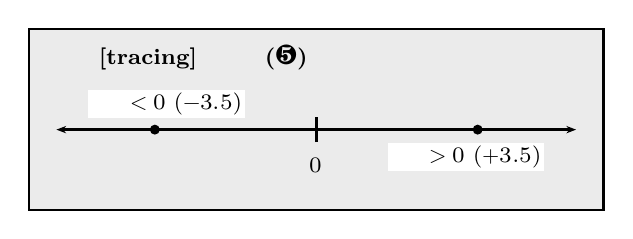
\begin{tikzpicture}[x=1cm, y=1cm, every node/.style={font=\footnotesize, text=black}]
      \draw[black, line width=0.85pt, fill=panelgray] (0,0) rectangle (7.30, 2.30);
      \node[anchor=north west] at (0.10, 2.22) {\textbf{ខ្សែអូស \en{[tracing]} ញែកសញ្ញា (\cnum{5})}};
      \draw[{Stealth[length=3.5pt]}-{Stealth[length=3.5pt]}, black, line width=1.0pt] (0.35, 1.02) -- (6.95, 1.02);
      \draw[black, line width=1.1pt] (3.65, 0.86) -- (3.65, 1.18);
      \node[below=2pt] at (3.65, 0.86) {$0$};
      \fill[black] (1.60, 1.02) circle (1.8pt);
      \node[above=3pt, fill=white, inner sep=1pt] at (1.75, 1.06) {ក្រុម $<0$ ($-3.5$)};
      \fill[black] (5.70, 1.02) circle (1.8pt);
      \node[below=3pt, fill=white, inner sep=1pt] at (5.55, 0.96) {ក្រុម $>0$ ($+3.5$)};
    \end{tikzpicture}
    \end{center}
    \begin{tcolorbox}[enhanced, sharp corners, colback=panelgray, colframe=black, boxrule=0.75pt, boxsep=1pt, top=4.5pt, bottom=4.5pt, left=5pt, right=5pt]
      \raggedright\fontsize{7.9pt}{11.2pt}\selectfont
      \textbf{ពិនិត្យក្រោយ (\en{EIA} ៣០ វិនាទី)៖}\\
      \textbf{១)} ហេតុអ្វី $-3\frac{1}{2}=-\frac{7}{2}$ មិនមែន $-\frac{5}{2}$? ($\underline{\hspace{2.3cm}}$)\\
      \textbf{២)} ហេតុអ្វីសៀវភៅភ្លេចផ្គុំ $3.5=\frac{21}{6}$ ហើយយើងត្រូវបំពេញបន្ថែម? ($\underline{\hspace{2.2cm}}$)
    \end{tcolorbox}
  \end{minipage}\hfill
  \begin{minipage}[t]{10.25cm}
    \vspace{0pt}
    \begin{tcolorbox}[enhanced, sharp corners, colback=white, colframe=black, boxrule=0.85pt, boxsep=1pt, top=5pt, bottom=5pt, left=5.5pt, right=5.5pt]
      \raggedright\fontsize{8.05pt}{11.8pt}\selectfont
      \textbf{ជំហាន ១–២ (គំរូ ១)៖ ញែកក្រុមសញ្ញា \cnum{5} \& បម្លែង \cnum{3} ទាំង ២ ក្រុម៖}\\[3.5pt]
      $\bullet$ \textbf{ក្រុមអវិជ្ជមាន ($<0$)៖} $-3\dfrac{1}{2} = -\left(3+\dfrac{1}{2}\right) = \dfrac{\fnum{0.55cm}}{2} = \dfrac{\fnum{0.60cm}}{4} = \underline{\hspace{0.85cm}}$ \chkbox\\[3.5pt]
      $\bullet$ \textbf{ក្រុមវិជ្ជមាន ($>0$ កែសៀវភៅខ្វះ!)៖} $3.5 = \dfrac{35}{10} = \dfrac{7}{2} = \dfrac{\fnum{0.55cm}}{6}$ \chkbox
    \end{tcolorbox}
    \vspace{6pt}
    \begin{tcolorbox}[enhanced, sharp corners, colback=panelgray, colframe=black, boxrule=0.85pt, boxsep=1pt, top=5pt, bottom=5pt, left=5.5pt, right=5.5pt]
      \raggedright\fontsize{8.05pt}{11.8pt}\selectfont
      \textbf{ជំហាន ៣ (គំរូ ២ ទំ.២)៖ កំណត់ $x$ ដើម្បីឱ្យ $\dfrac{45}{x}$ ស្មើ $7\dfrac{1}{2}$៖}\\[3.5pt]
      $\bullet$ \textbf{បម្លែង \cnum{3}៖} $7\dfrac{1}{2} = \dfrac{7\times 2+1}{2} = \dfrac{\fnum{0.55cm}}{2}$ \quad (លក្ខខណ្ឌ $x \neq \underline{\hspace{0.35cm}}$, \cnum{1})\\[3.5pt]
      $\bullet$ \textbf{ផលគុណខ្វែង \cnum{4}៖} $\dfrac{45}{x} = \dfrac{15}{2} \implies 15x = 2\times \underline{\hspace{0.55cm}} = \underline{\hspace{0.6cm}} \implies x = \underline{\hspace{0.5cm}}$ \chkbox
    \end{tcolorbox}
    \vspace{5pt}
    \raggedright{\fontsize{7.5pt}{10.5pt}\selectfont
    \textbf{ធនាគារ \cnum{1}–\cnum{5}៖} \cnum{1} $b\neq 0$ \en{|} \cnum{2} សញ្ញាដក \en{|} \cnum{3} ទម្រង់ ៥ \en{|} \cnum{4} $ad=bc$ \en{|} \cnum{5} ឆ្វេង/ស្ដាំ \en{0}\par}
  \end{minipage}
\end{tcolorbox}%
}

\vspace{4pt}
\eFourCardRN{ប័ណ្ណទី ១}

\vspace{14pt}
\noindent\scissors\ \dotfill\ \textbf{កាត់តាមស្នាមចុចចែកជា ២ ប័ណ្ណ (\en{Cut Along Dashed Line})} \dotfill\ \scissors
\vspace{14pt}

\eFourCardRN{ប័ណ្ណទី ២}

\clearpage

% ============================================================================
% ទំព័រទី ៣៖ E5 Evaluate — ២ សន្លឹក Relay ៣ តួនាទី «ប្រតិបត្តិ» (2-up)
% ============================================================================
\pagebanner{សម្ភារៈទី ៣៖ សន្លឹក \enbf{Relay 3} តួនាទី \enbf{–} «ប្រតិបត្តិ» \enbf{(}ទំ\enbf{.}២ \enbf{\&} បិទ \enbf{E1)}}{ទំព័រ ៣/៦ \en{– E5 Evaluate} (កាត់ ២ សន្លឹក \scissors)}

\newcommand{\eFiveSheetRN}[1]{%
\begin{tcolorbox}[
  enhanced, sharp corners, colback=white, colframe=white,
  borderline={1.0pt}{0pt}{black, dashed},
  boxsep=1pt, top=5pt, bottom=5pt, left=4.5pt, right=4.5pt
]
  \begin{tcolorbox}[
    enhanced, sharp corners, colback=headgray, colframe=black,
    boxrule=0.8pt, boxsep=1pt, top=3pt, bottom=3pt, left=5pt, right=5pt, after skip=4.5pt
  ]
    \fontsize{8.1pt}{11.2pt}\selectfont
    \textbf{\scissors\ សន្លឹក \en{Relay 3} តួនាទី (#1) \en{|} «ក្រុមវិស្វករសហគមន៍»} \hfill ក្រុម៖ $\underline{\hspace{2.4cm}}$\\[2pt]
    \textbf{ប្រតិបត្តិ (ទំ.២)៖} រក $x$ និង $y$ ដើម្បីឱ្យចំនួនសនិទាន $\dfrac{-2}{x},\; \dfrac{y}{5},\; -0.2$ ស្មើគ្នា (និងតេស្តសញ្ញា $-\dfrac{-5}{-1}$)~។
  \end{tcolorbox}

  \renewcommand{\arraystretch}{1.12}
  {\centering\setlength{\tabcolsep}{3.5pt}%
  \begin{tabular}{|L{6.15cm}|L{6.05cm}|L{5.25cm}|}
    \hline
    \cellcolor{panelgray}\centering\arraybackslash\fontsize{8.0pt}{10.6pt}\selectfont\textbf{តួនាទី ១៖ អ្នកអូសដាន \en{[tracing] \& Pause-Ask}}\newline {\fontsize{7.6pt}{10.2pt}\selectfont បម្លែង $-0.2$ និងពិនិត្យលក្ខខណ្ឌ $x \neq 0$} &
    \cellcolor{panelgray}\centering\arraybackslash\fontsize{8.0pt}{10.6pt}\selectfont\textbf{តួនាទី ២៖ អ្នកគណនា $x, y$ (\cnum{4})}\newline {\fontsize{7.6pt}{10.2pt}\selectfont ប្រើផលគុណខ្វែង $\frac{a}{b}=\frac{c}{d} \iff ad=bc$} &
    \cellcolor{panelgray}\centering\arraybackslash\fontsize{8.0pt}{10.6pt}\selectfont\textbf{តួនាទី ៣៖ \en{Pause-Review} \& បិទ \en{E1}}\newline {\fontsize{7.6pt}{10.2pt}\selectfont រាប់សញ្ញាដក \cnum{2} និងបិទទីផ្សារកំពង់ស្វាយ} \\ \hline

    % --- Col 1 ---
    \fontsize{8.0pt}{11.5pt}\selectfont
    \textbf{១) \en{[tracing]} បម្លែងទសភាគ \cnum{3}៖}\par\vspace{2.5pt}
    $-0.2 = \dfrac{\fnum{0.60cm}}{10} = \dfrac{\fnum{0.60cm}}{5}$\par\vspace{3.5pt}
    \textbf{២) ពិនិត្យលក្ខខណ្ឌ \cnum{1}, \cnum{5}៖}\par\vspace{2.5pt}
    $\bullet$ $x \neq \underline{\hspace{0.45cm}}$ (ភាគបែងហាមសូន្យ)\par\vspace{2.5pt}
    \chkbox\ \textbf{\en{Pause-Ask!}} ដោយភាគយក $-2 < 0$ និង $-0.2 < 0$ តើ $x$ ត្រូវមានសញ្ញាអ្វី? \quad \chkbox~$>0$ \quad \chkbox~$<0$
    &
    % --- Col 2 ---
    \fontsize{8.0pt}{11.5pt}\selectfont
    \textbf{១) រកតម្លៃ $x$ តាម \cnum{4}៖}\par\vspace{2.5pt}
    $\dfrac{-2}{x} = \dfrac{-1}{5} \implies (-1)x = (-2)\times 5$\par\vspace{2.5pt}
    $\implies -x = \underline{\hspace{0.65cm}} \implies x = \underline{\hspace{0.60cm}} \neq 0$ \chkbox\par\vspace{3.5pt}
    \textbf{២) រកតម្លៃ $y$ តាម \cnum{4}៖}\par\vspace{2.5pt}
    $\dfrac{y}{5} = \dfrac{-1}{5} \implies 5y = \underline{\hspace{0.65cm}} \implies y = \underline{\hspace{0.55cm}}$ \chkbox
    &
    % --- Col 3 ---
    \fontsize{7.9pt}{11.2pt}\selectfont
    \chkbox\ \textbf{\en{Pause-Review!}} រាប់សញ្ញាដក \cnum{2}៖\par\vspace{2pt}
    $-\dfrac{-5}{-1}$ មាន $\underline{\hspace{0.35cm}}$ សញ្ញាដក ($\square$ គត់ / $\square$ សេស) $\Rightarrow = \underline{\hspace{0.6cm}}$\par\vspace{3.5pt}
    \begin{tcolorbox}[enhanced, sharp corners, colback=panelgray, colframe=black, boxrule=0.7pt, boxsep=1pt, top=3.5pt, bottom=3.5pt, left=4.5pt, right=4.5pt]
      \raggedright\fontsize{7.6pt}{10.6pt}\selectfont
      \textbf{បិទបេសកកម្ម \en{E1} (កំពង់ស្វាយ)៖}\\
      $\bullet$ $3\div 6,\; -3,\; 0.5,\; 0.\overline{3} \in \underline{\hspace{0.5cm}}$ ($\frac{a}{b},\; b\neq 0$)!\\
      $\bullet$ តែ $4\div 0$ \textbf{ហាមចែក} ($\underline{\hspace{0.85cm}}$)!
    \end{tcolorbox}
    \\ \hline
  \end{tabular}\par}

  \vspace{4.5pt}
  {\centering
  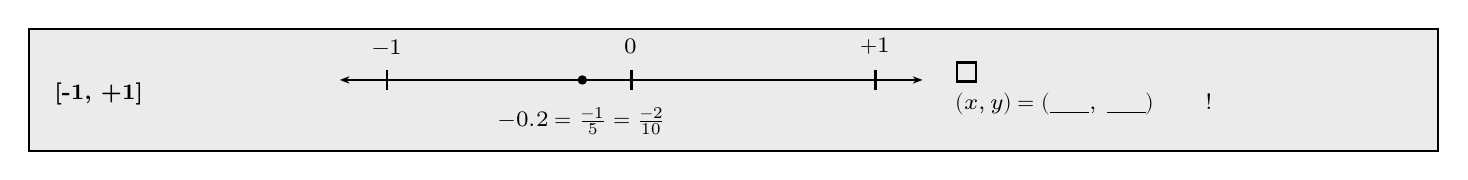
\begin{tikzpicture}[x=1cm, y=1cm, every node/.style={font=\footnotesize, text=black}]
    \draw[black, line width=0.8pt, fill=panelgray] (0,0) rectangle (17.90, 1.55);
    \node[anchor=west, align=left] at (0.20, 0.80) {\textbf{ផ្ទៀងជាប់បន្ទាត់}\\[1pt]\en{\textbf{[-1, +1]}}៖};
    \draw[{Stealth[length=3.5pt]}-{Stealth[length=3.5pt]}, black, line width=0.95pt] (3.95, 0.90) -- (11.35, 0.90);
    \draw[black, line width=1.0pt] (4.55, 0.77) -- (4.55, 1.03); \node[above=2pt] at (4.55, 1.03) {$-1$};
    \draw[black, line width=1.0pt] (7.65, 0.77) -- (7.65, 1.03); \node[above=2pt] at (7.65, 1.03) {$0$};
    \draw[black, line width=1.0pt] (10.75, 0.77) -- (10.75, 1.03); \node[above=2pt] at (10.75, 1.03) {$+1$};
    \fill[black] (7.03, 0.90) circle (1.7pt);
    \node[below=2pt] at (7.03, 0.75) {$-0.2 = \frac{-1}{5} = \frac{-2}{10}$};
    \node[anchor=west, align=left] at (11.65, 0.80) {\chkbox\ ទាំង ៣ នាក់ពិនិត្យ\\ $(x,y) = (\underline{\hspace{0.50cm}},\; \underline{\hspace{0.50cm}})$ រួចរាល់!};
  \end{tikzpicture}\par}
\end{tcolorbox}%
}

\vspace{4pt}
\eFiveSheetRN{សន្លឹកទី ១}

\vspace{14pt}
\noindent\scissors\ \dotfill\ \textbf{កាត់តាមស្នាមចុចចែកជា ២ សន្លឹក (\en{Cut Along Dashed Line})} \dotfill\ \scissors
\vspace{14pt}

\eFiveSheetRN{សន្លឹកទី ២}

\clearpage

% ============================================================================
% ទំព័រទី ៤៖ ផ្ទាំងសំអាងគោល ១ — សញ្ញាណចំនួនសនិទាន & ធនាគារហេតុផល ①–⑤
% ============================================================================
\begin{tcolorbox}[
  enhanced, sharp corners, colback=white, colframe=black,
  boxrule=1.5pt, borderline={0.6pt}{2.2pt}{black},
  boxsep=1pt, top=14pt, bottom=14pt, left=7pt, right=7pt
]
  \begin{center}
    {\fontsize{8.8pt}{12.0pt}\selectfont មន្ទីរអប់រំ យុវជន និងកីឡា ខេត្តកំពង់ធំ \en{|} ការិយាល័យអប់រំ យុវជន និងកីឡា ស្រុកកំពង់ស្វាយ \en{|} អនុវិទ្យាល័យព្រះក្រសាំង}\\[4pt]
    {\muol\fontsize{12.5pt}{18pt}\selectfont ផ្ទាំងសំអាងគោល ១៖ សញ្ញាណចំនួនសនិទាន និងធនាគារហេតុផល \enbf{(}\cnum{1}\enbf{–}\cnum{5}\enbf{)}}\\[4pt]
    {\fontsize{8.5pt}{11.5pt}\selectfont គណិតវិទ្យា ថ្នាក់ទី៨ \en{–} មេរៀនទី១ (ទំ.១\en{–}២) \en{|} គ្រូបង្រៀន៖ ហុក ប៊ុនថែន \en{|} ថ្ងៃចន្ទ ៨រោច ខែអស្សុជ ឆ្នាំមមី អដ្ឋស័ក ព.ស. ២៥៧០ (ទី២ វិច្ឆិកា ២០២៦)}\\[6pt]
    \khmflourish
  \end{center}
  \vspace{10pt}

  % --- ផ្នែកទី ១៖ និយមន័យ + វិធាន ad=bc + ២ កំណែប្រុងប្រយ័ត្ន (ឆ្វេង) & Hub-and-Spoke 5 ទម្រង់ (ស្ដាំ) ---
  \noindent
  \begin{minipage}[t]{8.55cm}
    \begin{tcolorbox}[enhanced, sharp corners, colback=panelgray, colframe=black, boxrule=0.95pt, boxsep=1pt, equal height group=posterTopRN, top=10pt, bottom=10pt, left=6pt, right=6pt]
      \raggedright\fontsize{8.8pt}{13.0pt}\selectfont
      \textbf{១. និយមន័យចំនួនសនិទាន (ទំ.១)៖}\\[3pt]
      ចំនួនសនិទានជាចំនួនដែលមានទម្រង់ $\dfrac{a}{b}$ ដែល $a, b \in \mathbb{Z}$ និង \textbf{$b \neq 0$} ។ \textit{(ឧ. $\frac{0}{4}=0$ តែ $\frac{4}{0}$ គ្មានន័យ!)}\\[8pt]
      \textbf{២. វិធានសមភាពចំនួនសនិទាន (ទំ.២ កែបន្ថែម $b,d\neq 0$)៖}\\[3pt]
      ចំពោះ $b \neq 0,\; d \neq 0$៖ \quad $\boxed{\dfrac{a}{b} = \dfrac{c}{d} \iff ad = bc}$\\[8pt]
      \textbf{៣. កំណត់សម្គាល់បង្ការអន្ទាក់ទាំង ២ (\en{Nuances \#1–2})៖}\\[3pt]
      $\bullet$ \textbf{ទសភាគដាច់ vs ខួប៖} ប្រភាគសម្រួលរួចចែកដាច់ \textbf{លុះត្រា} ភាគបែងមានតែកត្តាបឋម $\{2,5\}$ (ឧ. $\frac{1}{2}=0.5$); បើមានកត្តាផ្សេង (ដូច $3$, ឬ $163$ ក្នុង $\frac{17}{652}$) ទើបខួប ($\frac{1}{3}=0.\overline{3}$)!\\[4pt]
      $\bullet$ \textbf{ចំនួនចំរុះដក៖} $-3\dfrac{1}{4} = -\!\left(3+\dfrac{1}{4}\right) = \dfrac{-13}{4}$ \mbox{(\textbf{ហាម} $\frac{-3\times 4+1}{4}=\frac{-11}{4}$)}។
    \end{tcolorbox}
  \end{minipage}\hfill
  \begin{minipage}[t]{9.15cm}
    \begin{tcolorbox}[enhanced, sharp corners, colback=white, colframe=black, boxrule=0.95pt, boxsep=1pt, equal height group=posterTopRN, top=10pt, bottom=10pt, left=5pt, right=5pt]
      \centering
      \textbf{\fontsize{8.9pt}{12.2pt}\selectfont ដ្យាក្រាម \en{Hub-and-Spoke}៖ ទម្រង់ទាំង ៥ នៃ $\mathbb{Q}$ (\en{Xu et al., 2026})}\\[8pt]
      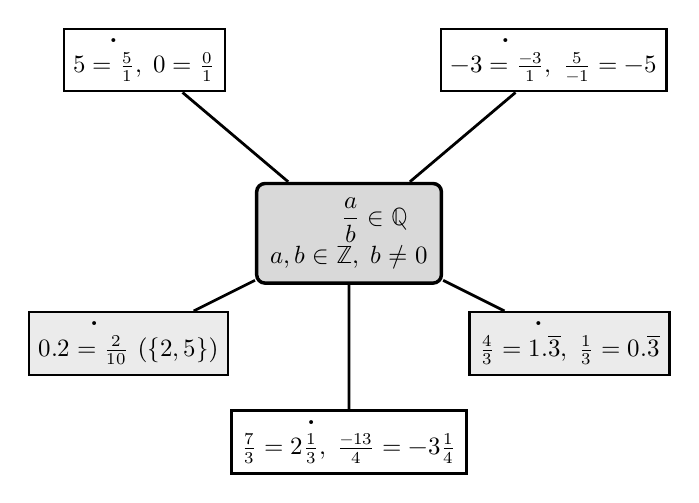
\begin{tikzpicture}[x=1cm, y=1cm, every node/.style={font=\small, text=black}]
        % Center Hub
        \node[draw=black, line width=1.25pt, fill=headgray, rounded corners=3pt, inner sep=5pt, align=center] (HUB) at (4.15, 2.95) {\textbf{ស្នូល៖} $\dfrac{a}{b}\in\mathbb{Q}$\\ $a,b\in\mathbb{Z},\; b\neq 0$};
        % 5 Spokes cleanly spaced
        \node[draw=black, line width=0.9pt, fill=white, inner sep=3.5pt, align=center] (S1) at (1.55, 5.15) {\textbf{១. ចំនួនគត់}\\ $5=\frac{5}{1},\; 0=\frac{0}{1}$};
        \node[draw=black, line width=0.9pt, fill=white, inner sep=3.5pt, align=center] (S2) at (6.75, 5.15) {\textbf{២. គត់រ៉ឺឡាទីបដក}\\ $-3=\frac{-3}{1},\; \frac{5}{-1}=-5$};
        \node[draw=black, line width=0.9pt, fill=panelgray, inner sep=3.5pt, align=center] (S3) at (1.35, 1.55) {\textbf{៣. ទសភាគដាច់}\\ $0.2=\frac{2}{10}$ ($\{2,5\}$)};
        \node[draw=black, line width=0.9pt, fill=panelgray, inner sep=3.5pt, align=center] (S4) at (6.95, 1.55) {\textbf{៤. ទសភាគខួប}\\ $\frac{4}{3}=1.\overline{3},\; \frac{1}{3}=0.\overline{3}$};
        \node[draw=black, line width=0.9pt, fill=white, inner sep=3.5pt, align=center] (S5) at (4.15, 0.30) {\textbf{៥. ចំនួនចំរុះ}\\ $\frac{7}{3}=2\frac{1}{3},\; \frac{-13}{4}=-3\frac{1}{4}$};
        \draw[black, line width=1.0pt] (HUB) -- (S1) (HUB) -- (S2) (HUB) -- (S3) (HUB) -- (S4) (HUB) -- (S5);
      \end{tikzpicture}
    \end{tcolorbox}
  \end{minipage}

  \vspace{14pt}

  % --- ផ្នែកទី ២៖ តារាងធនាគារហេតុផល ①–⑤ (១០០% ត្រូវគ្នានឹង LS_Plan_RN1) ---
  \fontsize{8.7pt}{12.5pt}\selectfont
  \renewcommand{\arraystretch}{1.72}
  \begin{tabular}{|C{0.75cm}|L{4.25cm}|L{7.15cm}|C{4.10cm}|}
    \hline
    \cellcolor{headgray}\textbf{លេខ} &
    \cellcolor{headgray}\centering\arraybackslash\textbf{ឈ្មោះហេតុផល} &
    \cellcolor{headgray}\centering\arraybackslash\textbf{និមិត្តសញ្ញា និងរបៀបប្រើក្នុងលំហាត់} &
    \cellcolor{headgray}\centering\arraybackslash\textbf{គំរូរូបសម្គាល់ ស-ខ្មៅ} \\ \hline

    \cnum{1} &
    \textbf{និយមន័យ $\frac{a}{b}\;(b\neq 0)$} &
    ពិនិត្យលក្ខខណ្ឌ $a, b \in \mathbb{Z}$ និងភាគបែង $b \neq 0$ មុនដោះស្រាយអញ្ញាត ($\frac{0}{4}=0$ តែ $\frac{4}{0}$ គ្មានន័យ)។ &
    \raisebox{-0.35\height}{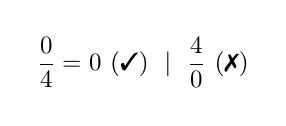
\begin{tikzpicture}[x=1cm, y=1cm, every node/.style={font=\small, text=black}]
      \node at (1.85, 0.28) {$\dfrac{0}{4}=0$ (\ding{51}) \;\textbar{}\; $\dfrac{4}{0}$ (\ding{55})};
    \end{tikzpicture}} \\ \hline

    \cnum{2} &
    \textbf{ច្បាប់សញ្ញា និងរាប់ដក} &
    $-\dfrac{a}{b}=\dfrac{-a}{b}=\dfrac{a}{-b}$ និង $\dfrac{-a}{-b}=\dfrac{a}{b}$ (រាប់សញ្ញាដក៖ គូ $\to +$, សេស $\to -$ លើ \#1, ប្រតិបត្តិ)។ &
    \raisebox{-0.35\height}{\begin{tikzpicture}[x=1cm, y=1cm, every node/.style={font=\small, text=black}]
      \node at (1.85, 0.28) {$-\dfrac{-5}{-1} \to 3$ ដក $= -5$};
    \end{tikzpicture}} \\ \hline

    \cnum{3} &
    \textbf{បម្លែងទម្រង់ ៥ យ៉ាង} &
    $n=\frac{n}{1}$; ទសភាគដាច់ $\frac{a}{10^k}$ ($\{2,5\}$); ខួប (កត្តាផ្សេងពី $\{2,5\}$); $\pm m\frac{p}{q}=\pm(m+\frac{p}{q})$។ &
    \raisebox{-0.35\height}{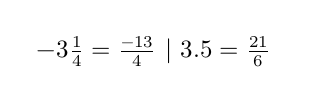
\begin{tikzpicture}[x=1cm, y=1cm, every node/.style={font=\small, text=black}]
      \node at (1.85, 0.28) {$-3\frac{1}{4}=\frac{-13}{4}$ \textbar{} $3.5=\frac{21}{6}$};
    \end{tikzpicture}} \\ \hline

    \cnum{4} &
    \textbf{វិធានផលគុណខ្វែង $ad=bc$} &
    ចំពោះ $b, d \neq 0$៖ $\dfrac{a}{b}=\dfrac{c}{d} \iff ad=bc$ (គំរូ ២ $x=6$, ប្រតិបត្តិ $x=10, y=-1$)។ &
    \raisebox{-0.35\height}{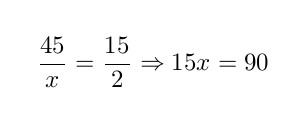
\begin{tikzpicture}[x=1cm, y=1cm, every node/.style={font=\small, text=black}]
      \node at (1.85, 0.28) {$\dfrac{45}{x}=\dfrac{15}{2} \Rightarrow 15x=90$};
    \end{tikzpicture}} \\ \hline

    \cnum{5} &
    \textbf{សញ្ញាឆ្វេង/ស្ដាំ ០ \en{[tracing]}} &
    ចំនួនអវិជ្ជមាន ($<0$, ឆ្វេង $0$) និងចំនួនវិជ្ជមាន ($>0$, ស្ដាំ $0$) មិនស្មើគ្នាឡើយ! &
    \raisebox{-0.35\height}{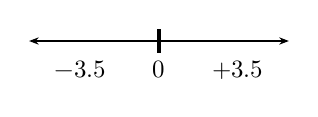
\begin{tikzpicture}[x=1cm, y=1cm, every node/.style={font=\small, text=black}]
      \draw[{Stealth[length=3.5pt]}-{Stealth[length=3.5pt]}, black, line width=1.0pt] (0.20,0.24) -- (3.50,0.24);
      \draw[black, line width=1.1pt] (1.85,0.09) -- (1.85,0.39);
      \node[below=1.5pt] at (0.85,0.16) {$-3.5$};
      \node[below=1.5pt] at (1.85,0.16) {$0$};
      \node[below=1.5pt] at (2.85,0.16) {$+3.5$};
    \end{tikzpicture}} \\ \hline
  \end{tabular}

  \vspace{14pt}
  \begin{tcolorbox}[enhanced, sharp corners, colback=panelgray, colframe=black, boxrule=0.85pt, boxsep=1pt, top=7pt, bottom=7pt, left=7pt, right=7pt]
    \centering\fontsize{8.7pt}{12.4pt}\selectfont
    \textbf{គោលការណ៍ប្រើផ្ទាំងសំអាងក្នុងថ្នាក់ (\en{E3–E5})៖} រាល់ការផ្គុំ ការបម្លែង និងការរកអញ្ញាត $x, y$ ក្នុង \textbf{គំរូទី ១–២ (ទំ.២)}, \textbf{ប្រតិបត្តិ (ទំ.២)} និង \textbf{លំហាត់ទំ.១១ (\#1, \#3, \#4)} ត្រូវភ្ជាប់លេខហេតុផល \cnum{1}–\cnum{5} ជានិច្ច!
  \end{tcolorbox}
\end{tcolorbox}

\clearpage

% ============================================================================
% ទំព័រទី ៥៖ កាតវិនិច្ឆ័យរហ័ស A–D & សំបុត្រចេញ ៣ សំណួរ — E5 Evaluate
% ============================================================================
\pagebanner{សម្ភារៈទី ៥៖ កាតវិនិច្ឆ័យរហ័ស «កាត \enbf{A–D}» \enbf{\&} សំបុត្រចេញ ៣ សំណួរ \enbf{E5}}{ទំព័រ ៥/៦ \en{– E5 Evaluate}}

{\fontsize{8.4pt}{11.8pt}\selectfont
\textbf{វិធីលេងក្នុងថ្នាក់៖} គ្រូលើកកាតម្ដងមួយ $\rightarrow$ សិស្សផ្ទៀងជាមួយ \cnum{1}–\cnum{5} $\rightarrow$ លើក \textbf{មេដៃឡើង (ពិត \ding{51})} ឬ \textbf{ខ្វែងដៃ (ខុស/អន្ទាក់ \ding{55})}!}

\vspace{6pt}

% --- ជួរទី ១៖ កាត A & កាត B ---
\noindent
\begin{tcolorbox}[
  enhanced, sharp corners, colback=white, colframe=white,
  borderline={1.0pt}{0pt}{black, dashed},
  width=9.25cm, equal height group=rnfoilrow1, nobeforeafter,
  boxsep=1pt, top=6pt, bottom=6pt, left=6pt, right=6pt
]
  \noindent\colorbox{black}{\textcolor{white}{\Large\textbf{\en{ A }}}}\hspace{0.22cm}{\fontsize{9.0pt}{12.2pt}\selectfont\textbf{កាត \en{A} ៖ បម្លែងទម្រង់ចំនួនចំរុះដក}}\par\vspace{6pt}
  \begin{center}
  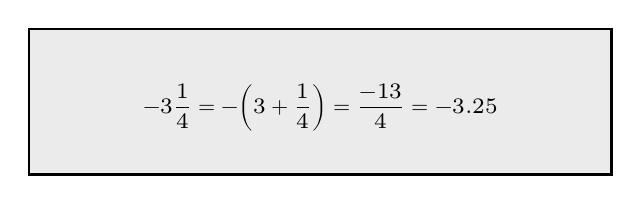
\begin{tikzpicture}[x=1cm, y=1cm, every node/.style={font=\footnotesize, text=black}]
    \draw[black, line width=1.0pt, fill=panelgray] (0,0) rectangle (7.40, 1.85);
    \node[align=center] at (3.70, 0.925) {\textbf{ការអះអាង៖}\\[3pt]
      $-3\dfrac{1}{4} = -\!\left(3 + \dfrac{1}{4}\right) = \dfrac{-13}{4} = -3.25$};
  \end{tikzpicture}
  \end{center}
  \vfill
  \begin{tcolorbox}[enhanced, sharp corners, colback=panelgray, colframe=black, boxrule=0.8pt, boxsep=1pt, top=4pt, bottom=4pt, left=4pt, right=4pt]
    \centering\fontsize{8.7pt}{11.8pt}\selectfont
    \textbf{សំណួរ៖} ត្រឹមត្រូវឬទេ? \quad \chkbox~ពិត (\ding{51}) \quad \chkbox~ខុស (\ding{55})
  \end{tcolorbox}
\end{tcolorbox}%
\hfill
\begin{tcolorbox}[
  enhanced, sharp corners, colback=white, colframe=white,
  borderline={1.0pt}{0pt}{black, dashed},
  width=9.25cm, equal height group=rnfoilrow1, nobeforeafter,
  boxsep=1pt, top=6pt, bottom=6pt, left=6pt, right=6pt
]
  \noindent\colorbox{black}{\textcolor{white}{\Large\textbf{\en{ B }}}}\hspace{0.22cm}{\fontsize{9.0pt}{12.2pt}\selectfont\textbf{កាត \en{B} ៖ អន្ទាក់ភាគបែងសូន្យ ($b=0$)}}\par\vspace{6pt}
  \begin{center}
  
\begin{tikzpicture}[x=1cm, y=1cm, every node/.style={font=\footnotesize, text=black}]
    \draw[black, line width=1.0pt, fill=panelgray] (0,0) rectangle (7.40, 1.85);
    \node[align=center] at (3.70, 0.925) {\textbf{ការអះអាង៖}\\[3pt]
      $\dfrac{4}{0} = 0$ គឺជាចំនួនសនិទាន!};
  \end{tikzpicture}
  \end{center}
  \vfill
  \begin{tcolorbox}[enhanced, sharp corners, colback=panelgray, colframe=black, boxrule=0.8pt, boxsep=1pt, top=4pt, bottom=4pt, left=4pt, right=4pt]
    \centering\fontsize{8.7pt}{11.8pt}\selectfont
    \textbf{សំណួរ៖} ត្រឹមត្រូវឬទេ? \quad \chkbox~ពិត (\ding{51}) \quad \chkbox~ខុស (\ding{55})
  \end{tcolorbox}
\end{tcolorbox}

\vspace{7pt}

% --- ជួរទី ២៖ កាត C & កាត D ---
\noindent
\begin{tcolorbox}[
  enhanced, sharp corners, colback=white, colframe=white,
  borderline={1.0pt}{0pt}{black, dashed},
  width=9.25cm, equal height group=rnfoilrow2, nobeforeafter,
  boxsep=1pt, top=6pt, bottom=6pt, left=6pt, right=6pt
]
  \noindent\colorbox{black}{\textcolor{white}{\Large\textbf{\en{ C }}}}\hspace{0.22cm}{\fontsize{9.0pt}{12.2pt}\selectfont\textbf{កាត \en{C} ៖ កាត់ចោលគត់ និងទសភាគខួប}}\par\vspace{6pt}
  \begin{center}
  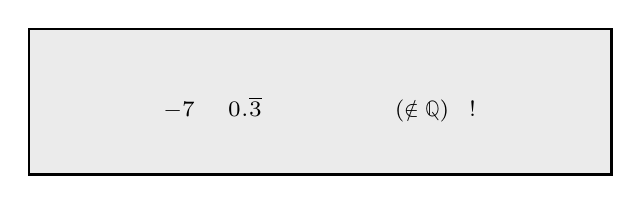
\begin{tikzpicture}[x=1cm, y=1cm, every node/.style={font=\footnotesize, text=black}]
    \draw[black, line width=1.0pt, fill=panelgray] (0,0) rectangle (7.40, 1.85);
    \node[align=center] at (3.70, 0.925) {\textbf{ការអះអាង៖}\\[3pt]
      $-7$ និង $0.\overline{3}$ \textbf{មិនមែន}ជាចំនួនសនិទាន ($\notin \mathbb{Q}$) ទេ!};
  \end{tikzpicture}
  \end{center}
  \vfill
  \begin{tcolorbox}[enhanced, sharp corners, colback=panelgray, colframe=black, boxrule=0.8pt, boxsep=1pt, top=4pt, bottom=4pt, left=4pt, right=4pt]
    \centering\fontsize{8.7pt}{11.8pt}\selectfont
    \textbf{សំណួរ៖} ត្រឹមត្រូវឬទេ? \quad \chkbox~ពិត (\ding{51}) \quad \chkbox~ខុស (\ding{55})
  \end{tcolorbox}
\end{tcolorbox}%
\hfill
\begin{tcolorbox}[
  enhanced, sharp corners, colback=white, colframe=white,
  borderline={1.0pt}{0pt}{black, dashed},
  width=9.25cm, equal height group=rnfoilrow2, nobeforeafter,
  boxsep=1pt, top=6pt, bottom=6pt, left=6pt, right=6pt
]
  \noindent\colorbox{black}{\textcolor{white}{\Large\textbf{\en{ D }}}}\hspace{0.22cm}{\fontsize{9.0pt}{12.2pt}\selectfont\textbf{កាត \en{D} ៖ អន្ទាក់ \en{\textit{Negz}} និងចំរុះដក}}\par\vspace{6pt}
  \begin{center}
  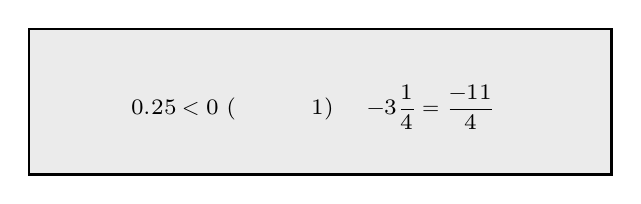
\begin{tikzpicture}[x=1cm, y=1cm, every node/.style={font=\footnotesize, text=black}]
    \draw[black, line width=1.0pt, fill=panelgray] (0,0) rectangle (7.40, 1.85);
    \node[align=center] at (3.70, 0.925) {\textbf{ការអះអាង៖}\\[3pt]
      $0.25 < 0$ (ព្រោះតូចជាង $1$) និង $-3\dfrac{1}{4} = \dfrac{-11}{4}$~។};
  \end{tikzpicture}
  \end{center}
  \vfill
  \begin{tcolorbox}[enhanced, sharp corners, colback=panelgray, colframe=black, boxrule=0.8pt, boxsep=1pt, top=4pt, bottom=4pt, left=4pt, right=4pt]
    \centering\fontsize{8.7pt}{11.8pt}\selectfont
    \textbf{សំណួរ៖} ត្រឹមត្រូវឬទេ? \quad \chkbox~ពិត (\ding{51}) \quad \chkbox~ខុស (\ding{55})
  \end{tcolorbox}
\end{tcolorbox}

\vspace{7pt}

% --- ផ្នែកទី ៣៖ ចម្លើយគ្រូ (កាត A–D + Exit Ticket Key) & សំបុត្រចេញ ២ ប័ណ្ណសម្រាប់សិស្ស ---
\noindent\scissors\ \dotfill\ \textbf{កាត់ទុកសម្រាប់គ្រូ (\en{Teacher Key – Cards A–D \& Exit Ticket})} \dotfill\ \scissors

\vspace{4pt}
\begin{tcolorbox}[
  enhanced, sharp corners, colback=panelgray, colframe=black,
  boxrule=0.95pt, boxsep=1pt, top=4pt, bottom=4pt, left=5pt, right=5pt
]
  \fontsize{7.8pt}{10.9pt}\selectfont
  \renewcommand{\arraystretch}{1.12}
  \begin{tabular}{|L{4.25cm}|L{4.25cm}|L{4.25cm}|L{4.25cm}|}
    \hline
    \cellcolor{headgray}\textbf{កាត \en{A} ៖ មេដៃឡើង (\ding{51})} &
    \cellcolor{headgray}\textbf{កាត \en{B} ៖ ខ្វែងដៃ (\ding{55})} &
    \cellcolor{headgray}\textbf{កាត \en{C} ៖ ខ្វែងដៃ (\ding{55})} &
    \cellcolor{headgray}\textbf{កាត \en{D} ៖ ខ្វែងដៃ (\ding{55})} \\ \hline
    \textbf{ពិត!} $-3\frac{1}{4}=-\left(3+\frac{1}{4}\right)=\frac{-13}{4}=-3.25$ តាម \cnum{3}។ &
    \textbf{អន្ទាក់ $b=0$!} $\frac{4}{0}=k \iff k\times 0=4$ គ្មាន $k \Rightarrow$ គ្មានន័យ (\cnum{1})! &
    \textbf{កាត់ចោលខុស!} $-7=\frac{-7}{1}$ និង $0.\overline{3}=\frac{1}{3}$ សុទ្ធតែ $\in \mathbb{Q}$! &
    \textbf{ខុស \en{\textit{Negz}} \& ចំរុះ!} $0.25>0$ ស្ដាំ $0$ (\cnum{5}) និង $-3\frac{1}{4}=\frac{-13}{4}\neq \frac{-11}{4}$! \\ \hline
  \end{tabular}\\[3.5pt]
  \textbf{ចម្លើយសំបុត្រចេញសម្រាប់គ្រូ (\en{Exit Ticket Key})៖} \textbf{១)} $-2\frac{3}{4} = \mathbf{\frac{-11}{4} = -2.75}$ \;\textbar{}\; \textbf{២)} $\frac{0}{-5}=\mathbf{0\in\mathbb{Q}}$ តែ $\frac{-5}{0}$ គ្មានន័យ ($b\neq 0$) \;\textbar{}\; \textbf{៣)} $12\div m=-0.6 \Rightarrow \mathbf{m=-20\neq 0}$។
\end{tcolorbox}

\newcommand{\exitTicketSlipRN}[1]{%
\begin{tcolorbox}[
  enhanced, sharp corners, colback=white, colframe=white,
  borderline={0.95pt}{0pt}{black, dashed},
  boxsep=1pt, top=5pt, bottom=5pt, left=6pt, right=6pt
]
  \raggedright\fontsize{8.1pt}{11.8pt}\selectfont
  \textbf{\scissors\ សំបុត្រចេញ ៣ សំណួរ (#1 – ៦០–៩០ វិនាទី)៖}\quad ឈ្មោះ៖ $\underline{\hspace{3.8cm}}$ \quad ថ្នាក់៖ $\underline{\hspace{1.3cm}}$\\[4pt]
  \textbf{១)} បម្លែង $-2\dfrac{3}{4}$ ជាប្រភាគ $\dfrac{a}{b}$ និងចំនួនទសភាគ៖ \quad $-2\dfrac{3}{4} = \dfrac{\fnum{0.70cm}}{4} = \underline{\hspace{1.1cm}}$\\[3.5pt]
  \textbf{២)} ក្នុង $\dfrac{0}{-5}$ និង $\dfrac{-5}{0}$ តើមួយណាជាចំនួនសនិទាន? $\underline{\hspace{1.2cm}}$ \quad ហេតុអ្វី? $\underline{\hspace{6.2cm}}$\\[3.5pt]
  \textbf{៣)} រក $m$ ដើម្បីឱ្យ $\dfrac{12}{m} = -0.6$៖ \quad $\dfrac{12}{m} = \dfrac{-3}{5} \implies m = \underline{\hspace{1.2cm}} \quad (m \neq 0)$
\end{tcolorbox}%
}

\vspace{5pt}
\noindent\scissors\ \dotfill\ \textbf{កាត់ចែកសិស្ស៖ សំបុត្រចេញ \en{2-up} (\en{Student Exit Tickets – Print Clean})} \dotfill\ \scissors
\vspace{4pt}

\exitTicketSlipRN{សន្លឹកទី ១}
\vspace{5pt}
\exitTicketSlipRN{សន្លឹកទី ២}

\clearpage

% ============================================================================
% ទំព័រទី ៦៖ ប័ណ្ណកិច្ចការផ្ទះ ជំហានទី ៥ — ៤ ប័ណ្ណក្នុង ១ ទំព័រ A4 (ទំ.១១: #1, #3(ក,គ), #4(ក–ង))
% ============================================================================
\pagebanner{សម្ភារៈទី ៦៖ ប័ណ្ណកិច្ចការផ្ទះ ជំហានទី ៥ \enbf{(}ទំ\enbf{.}១១\enbf{)} \enbf{–} ៤ ប័ណ្ណក្នុង ១ ទំព័រ \enbf{A4}}{ទំព័រ ៦/៦ \en{–} ជំហានទី ៥ (កាត់ ៤ ប័ណ្ណ \scissors)}

% ប្រយ័ត្ន៖ កុំសរសេរ #1 ជាប់លេខ 1..9! បង្ហាញលេខជាអក្សរខ្មែរឬដកឃ្លា
\newcommand{\hwslipFourRN}[1]{%
\begin{tcolorbox}[
  enhanced, sharp corners, colback=white, colframe=white,
  borderline={0.95pt}{0pt}{black, dashed},
  width=9.25cm, equal height group=hwquadRN, nobeforeafter,
  boxsep=1pt, top=6.5pt, bottom=6.5pt, left=5pt, right=5pt
]
  \begin{tcolorbox}[
    enhanced, sharp corners, colback=headgray, colframe=black,
    boxrule=0.75pt, boxsep=1pt, top=3pt, bottom=3pt, left=4.5pt, right=4.5pt, after skip=5.5pt
  ]
    \fontsize{7.9pt}{10.8pt}\selectfont
    \textbf{\scissors\ កិច្ចការផ្ទះ (#1) \en{|} ១. សញ្ញាណចំនួនសនិទាន} \hfill \textbf{ចន្ទ ០២/១១/២៦}\\[2.5pt]
    ឈ្មោះ៖ $\underline{\hspace{4.0cm}}$ \hspace{0.2cm} ថ្នាក់៖ $\underline{\hspace{1.0cm}}$
  \end{tcolorbox}

  \fontsize{7.9pt}{11.8pt}\selectfont
  \textbf{លំហាត់ទី ១ (ទំ.១១)៖} ក្នុងបណ្ដាប្រភាគខាងក្រោម តើណាខ្លះស្មើនឹង $-5$?\\[3pt]
  \centerline{$\dfrac{-5}{1},\quad \dfrac{5}{1},\quad \dfrac{5}{-1},\quad -\dfrac{5}{1},\quad \dfrac{-5}{-1},\quad -\dfrac{-5}{1},\quad -\dfrac{-5}{-1}$}\\[3pt]
  {\fontsize{7.6pt}{10.8pt}\selectfont\textit{គន្លឹះ \cnum{2}៖ រាប់សញ្ញាដក! សេស ($1, 3$ ដក) $= -5$; គូ ($0, 2$ ដក) $= +5$។}}

  \vspace{4.5pt}\hrule height 0.45pt\vspace{4.5pt}

  \textbf{លំហាត់ទី ៣ (ទំ.១១)៖} សរសេរជាប្រភាគ (បង្រួមជា \cnum{3})៖\\[3pt]
  \hspace*{0.3cm}\textbf{ក.} $28.45 = \dfrac{\fnum{1.05cm}}{\fden{1.05cm}}$ \qquad \textbf{គ.} $1\dfrac{19}{50} = \dfrac{\fnum{1.05cm}}{\fden{1.05cm}}$\\[3pt]
  {\fontsize{7.4pt}{10.4pt}\selectfont\textit{(កំណត់សម្គាល់៖ ខ. $1.37\overline{8}$, ឃ. $0.\overline{13}$, ង. $0.34\overline{7}$ ជាទសភាគខួបសម្រាប់ម៉ោងក្រោយ)}}

  \vspace{4.5pt}\hrule height 0.45pt\vspace{4.5pt}

  \textbf{លំហាត់ទី ៤ (ទំ.១១)៖} សរសេរប្រភាគខាងក្រោមជាចំនួនទសភាគ៖\\[3pt]
  \hspace*{0.2cm}\textbf{ក.} $\dfrac{7}{100} = \underline{\hspace{1.1cm}}$ \quad \textbf{ខ.} $\dfrac{13}{10,000} = \underline{\hspace{1.2cm}}$ \quad \textbf{គ.} $\dfrac{3}{2^4} = \underline{\hspace{1.1cm}}$\\[3pt]
  \hspace*{0.2cm}\textbf{ឃ.} $\dfrac{7}{2^3\cdot 5} = \underline{\hspace{1.1cm}}$ \quad \textbf{ង.} $\dfrac{17}{652} \approx \underline{\hspace{1.8cm}}$\\[3pt]
  {\fontsize{7.5pt}{10.6pt}\selectfont\textit{គន្លឹះ (ង)៖ $652 = 2^2 \times 163$ ($163 \notin \{2,5\}$ $\Rightarrow$ ទសភាគខួប!)}}

  \vspace{5pt}
  \begin{tcolorbox}[
    enhanced, sharp corners, colback=panelgray, colframe=black,
    boxrule=0.7pt, boxsep=1pt, top=3.5pt, bottom=3.5pt, left=4.5pt, right=4.5pt
  ]
    \fontsize{7.5pt}{10.4pt}\selectfont
    \textbf{ផ្ទៀងមុនចេញ៖} \chkbox~រាប់ដក \en{\#1} \en{|} \chkbox~បង្រួម \en{\#3} \en{|} \chkbox~កត្តា $\{2,5\}$ \en{\#4} \en{|} \textbf{អានមុន ២.១ (ទំ.២–៣)}
  \end{tcolorbox}
\end{tcolorbox}%
}

\vspace{4pt}
\noindent
\hwslipFourRN{ប័ណ្ណទី ១}\hfill\hwslipFourRN{ប័ណ្ណទី ២}

\vspace{14pt}
\noindent\scissors\ \dotfill\ \textbf{កាត់តាមស្នាមចុចចែកជា ៤ ប័ណ្ណ (\en{Cut Along Dashed Lines})} \dotfill\ \scissors
\vspace{14pt}

\noindent
\hwslipFourRN{ប័ណ្ណទី ៣}\hfill\hwslipFourRN{ប័ណ្ណទី ៤}

\end{document}
